\chapter{Optimierung}
Im folgenden Abschnitt soll die mathematische Modellierung der Sozialen Hierarchie, der Beutesuche, deren Einkreisen und der Angriff vorgestellt werden.


\section{Soziale Hierarchie}
Für die Optimierung wird davon ausgegangen, dass Alpha-, Beta- und Deltawolf besten Kenntnisse über den Standort der Beute haben und sich das Rudel anhand deren Positionen ausrichtet. Dazu werden pro Runde die besten drei Lösungen ermittelt und entsprechend als Alpha, Beta und Delta klassifiziert. Alle übrigen Lösungen werden zu den Omegas gezählt und damit nicht weiter untergliedert. \\
Alpha, Beta und Delta führen die Jagd (Optimierung) an und alle übrigen Omegas folgen diesen. Pro Runde werden für jeden Wolf neue Positionen anhand der Positionen von Alpha, Beta und Delta berechnet und damit die Position Wölfe immer in eine bestimmte Richtung konvergiert. Durch die Anwendung von Limits kann das Rudel wieder zusammen gezogen werden, wenn sich die einzelnen Mitglieder zu weit verstreuen.

\section{Beutetier einkreisen}
Das Umkreisen der Beute wird mit folgenden Formeln beschrieben:
\begin{equation}
    \vec{D} = |\vec{C} \cdot \vec{X_p}(t) - \vec{X}(t) |
    \label{calcD}
\end{equation}
\begin{equation}
    \vec{X}(t+1) = \vec{X_p}(t) - \vec{A} \cdot \vec{D}
    \label{calcNextP}
\end{equation}

Wobei $t$ die momentane Iteration angibt und $\vec{A}$ und $\vec{C}$ Koeffizientenvekoren sind, $\vec{X_p}$ die Position der Beute (Prey) und $\vec{X}$ die Position eines Wolfes.\\
Der Vektor $\vec{D}$ (\autoref{calcD}) gibt die Richtung an, in die der Rest des Rudels konvergieren soll und wird zur Bestimmung des nächsten Positionsvektors eines Wolfes ($\vec{X}(t+1)$, \autoref{calcNextP}) gebraucht.\\
Die Vektoren $\vec{A}$ und $\vec{C}$ werden mit folgenden Formeln bestimmt:

\begin{equation}
    \vec{A} = 2 \vec{a} \cdot \vec{r_1} - \vec{a}
    \label{calcA}
\end{equation}
\begin{equation}
    \vec{C} = 2 \vec{r_2}
    \label{calcC}
\end{equation}

Die Komponenten von $\vec{a}$ werden mit jeder Iteration linear von $2$ bis $0$ verringert und $\vec{r_1}$ und $\vec{r_2}$ sind Zufallsvektoren in $[0,1]$.\\
\begin{figure}[ht]
    \begin{center}
        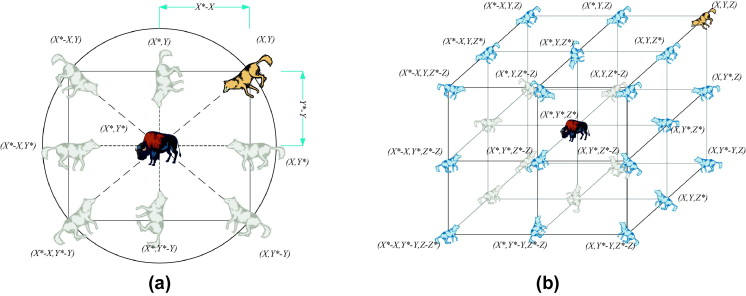
\includegraphics[width=0.7\textwidth]{assets/img/Updating_position_of_gray_wolves_in_GWO.jpg}
        \caption[Positionsneuberechnung im GWO]{Positionsneuberechnung im GWO \cite{MIRJALILI201446}}
        \label{gwo_newPos}
    \end{center}
\end{figure}

\section{Jagd}
\section{Beute angreifen}